\documentclass{article}
\usepackage{cmap}
\usepackage[utf8]{inputenc}
\usepackage[english,ukrainian]{babel}
\usepackage{graphicx}
\usepackage{geometry}
\usepackage{listings}
\usepackage{float}
\usepackage{amsmath}
\usepackage{subfig}
\geometry{
	a4paper,
	left=20mm,
	right=20mm,
	top=15mm,
	bottom=15mm,
}
\lstset{
	language=c,
	tabsize=4,
	keepspaces,
	showstringspaces=false,
}
\graphicspath{ {./pictures} }
\setlength{\parindent}{4em}

\newcommand\subject{Архітектура комп'ютера}
\newcommand\lecturer{доцент кафедри ПЗ\\Крук О.Г.}
\newcommand\teacher{доцент кафедри ПЗ\\Крук О.Г.}
\newcommand\mygroup{ПЗ-22}
\newcommand\lab{4}
\newcommand\theme{Синтез та моделювання основних типів регістрів та лічильників в системі Proteus}
\newcommand\purpose{Поглибити знання про будову та функціонування основних типів регістрів та лічильників; синтезувати їх схеми та виконати моделювання в системі програм Proteus; дослідити на основі отриманих часових діаграм їх роботу}

\begin{document}
\begin{normalsize}
	\begin{titlepage}
		\thispagestyle{empty}
		\begin{center}
			\textbf{МІНІСТЕРСТВО ОСВІТИ І НАУКИ УКРАЇНИ\\
				НАЦІОНАЛЬНИЙ УНІВЕРСИТЕТ "ЛЬВІВСЬКА ПОЛІТЕХНІКА"}
		\end{center}
		\begin{flushright}
			\textbf{ІКНІ}\\
			Кафедра \textbf{ПЗ}
		\end{flushright}
		\vspace{200pt}
		\begin{center}
			\textbf{ЗВІТ}\\
			\vspace{10pt}
			до лабораторної роботи № \lab\\
			\textbf{на тему}: “\textit{\theme}”\\
			\textbf{з дисципліни}: “\subject”
		\end{center}
		\vspace{112pt}
		\begin{flushright}
			
			\textbf{Лектор}:\\
			\lecturer\\
			\vspace{28pt}
			\textbf{Виконав}:\\
			
			студент групи \mygroup\\
			Коваленко Д.М.\\
			\vspace{28pt}
			\textbf{Прийняв}:\\
			
			\teacher\\
			
			\vspace{28pt}
			«\rule{1cm}{0.15mm}» \rule{1.5cm}{0.15mm} 2022 р.\\
			$\sum$ = \rule{1cm}{0.15mm}……………\\
			
		\end{flushright}
		\vspace{\fill}
		\begin{center}
			\textbf{Львів — 2022}
		\end{center}
	\end{titlepage}
		
	\begin{description}
		\item[Тема.] \theme.
		\item[Мета.] \purpose.
	\end{description}

	\section*{Індивідуальне завдання}
\begin{figure}[H]
		\centering
		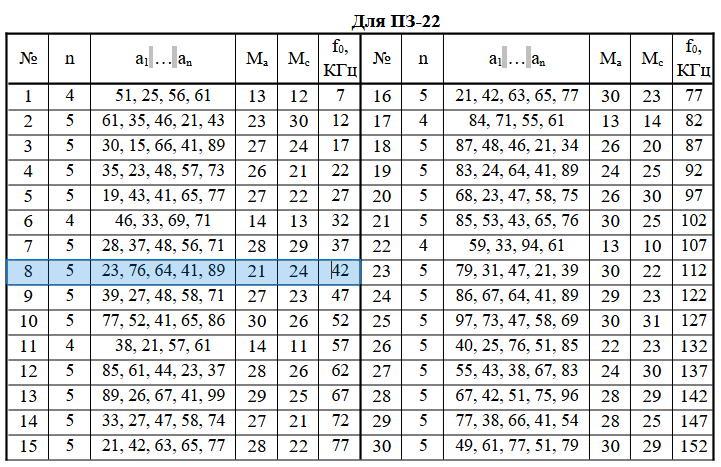
\includegraphics[scale=0.6]{v}
	\end{figure}	

	\section*{Теоретичні відомості}
	Регістр - це типовий функціональний вузол комп’ютера, призначений для приймання, тимчасового зберігання, перетворення і видавання n-розрядного двійкового слова. Регістр містить регулярний набір однотипових тригерів, в кожному з яких зберігається значення одного двійкового розряду машинного  слова. Найчастіше використовують тригери типів D, RS та JK.
	Регістри, призначені тільки для приймання (записування), зберігання і видавання інформації, називаються елементарними або регістрами пам’яті, або ж фіксаторами Регістри пам’яті - це пристрої з паралельним записуванням та зчитуванням інформації, яка подана в паралельному коді. Записана у тригери інформація може зчитуватись у прямому коді, інверсному або одночасно в прямому та інверсному кодах.
	
	Вони можуть бути синхронізовані рівнем або фронтом тактового сигналу залежно від типу застосовуваних тригерів. Елементарні регістри будують на одноступеневих тригерах. Логічна функція регістра позначається буквами RG (register).
	
	Регістри, в яких зберігання даних поєднується з мікроопераціями зсуву, називаються регістрами зсуву. Зсув – це одночасне просторове переміщення двійкового слова із збереженням порядку слідування нулів і одиниць. Мікрооперації зсуву використовують при виконанні команд множення, ділення та нормалізації. Крім того, за допомогою зсуву здійснюється перетворення паралельного коду в послідовний або навпаки. Зсув слова може виконуватися вправо (у бік молодших розрядів) або вліво (у бік старших розрядів). 
	
	Лічильник - це типовий функціональний вузол комп'ютера, призначений для лiчби та фіксації вхідних імпульсів. Лічильник складається із послідовно зв’язаних Т-тригерів, які утворюють пам’ять iз заданим числом сталих станів
	\section*{Хід роботи}
	\begingroup
	\setlength{\belowdisplayskip}{-15pt}
	\setlength{\abovedisplayskip}{0pt}
	\subsection*{Період цифрового сигналу}
	\begin{large}
		\begin{gather}
			T=\frac{1}{f};\hspace{22mm}T=\frac{1}{42\text{кГц}}=\frac{1}{42000\text{Гц}}=0.00002381\text{с}\nonumber\\
			\tau=\frac{T}{4}=0.000005952\text{с}\nonumber\\
			2\tau=2\cdot 0.000005952=0.0000119\text{c}\nonumber\\
			0.7\tau=0.7\cdot 0.000005952=0.000004167\text{c}\nonumber\\
			(2^n+1)\cdot T=(2^5+1)\cdot 0.00002381=0.0007857\text{c}\nonumber
		\end{gather}
	\end{large}
	\subsection*{Двійковий код заданих чисел $a_1$...$a_5$}
	\begin{large}
		\begin{gather}
			a_1=23_{10}=00010111_2\nonumber\\
			a_2=76_{10}=01001100_2\nonumber\\
			a_3=64_{10}=01000000_2\nonumber\\
			a_4=41_{10}=00101001_2\nonumber\\
			a_5=89_{10}=01011001_2\nonumber
		\end{gather}
	\end{large}
	\endgroup

	\section*{5-розрядний паралельний регістр пам'яті}	
	\begin{figure}[H]
		\centering
		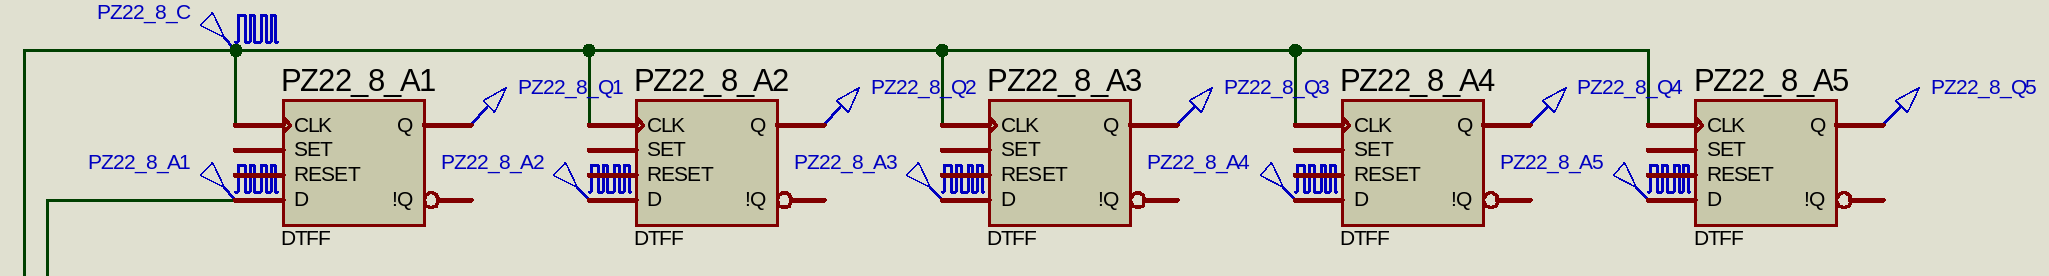
\includegraphics[scale=0.25]{s1}	
		\caption{Схема паралельного регістра}
	\end{figure}

	\begin{figure}[H]
		\centering
		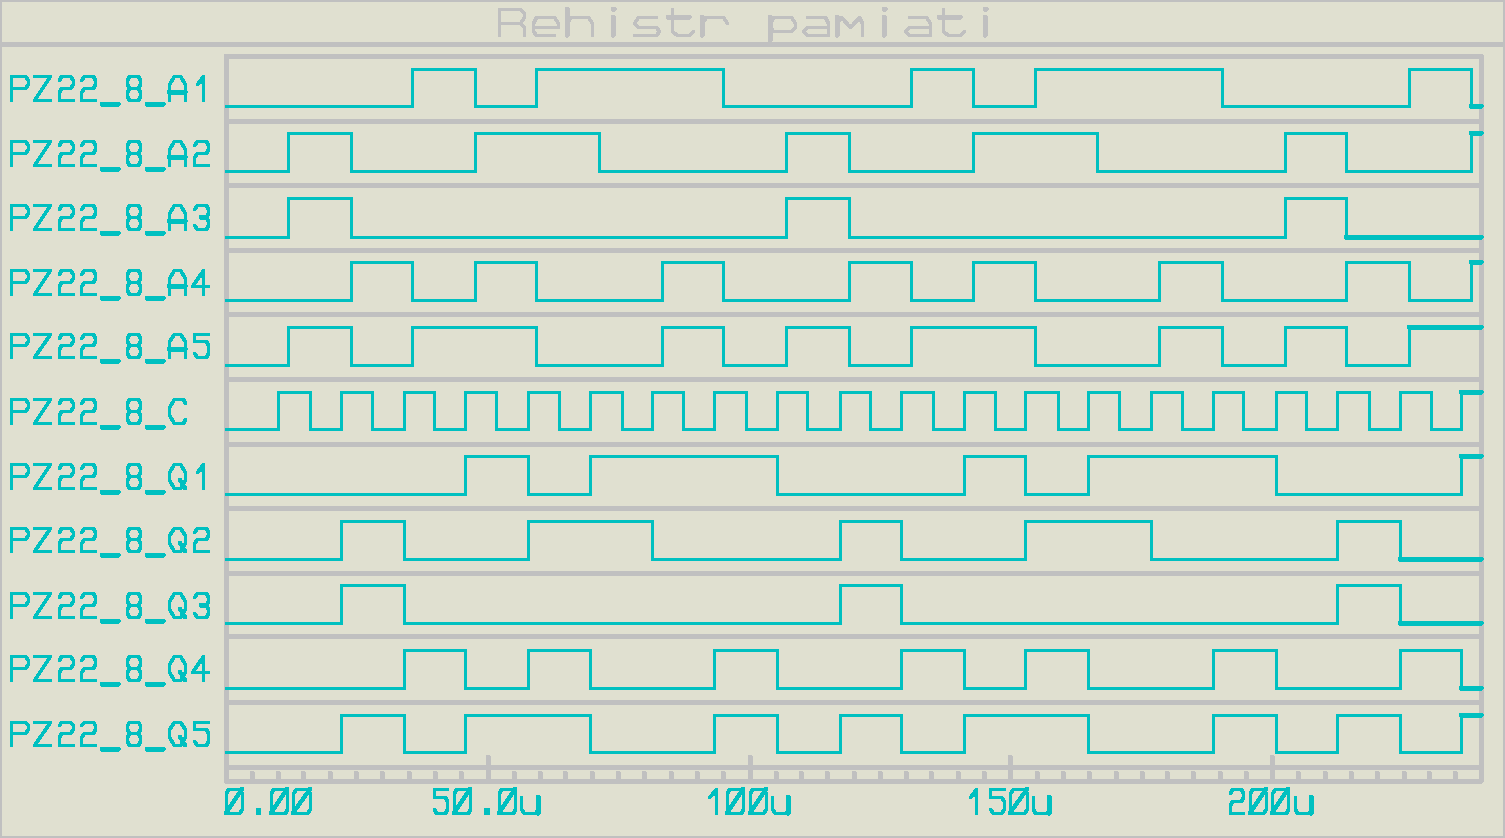
\includegraphics[scale=0.25]{g1}	
		\caption{Графік до схеми паралельного регістра}
	\end{figure}

	\begin{figure}[H]
		\centering
		\subfloat[Генератор C]{{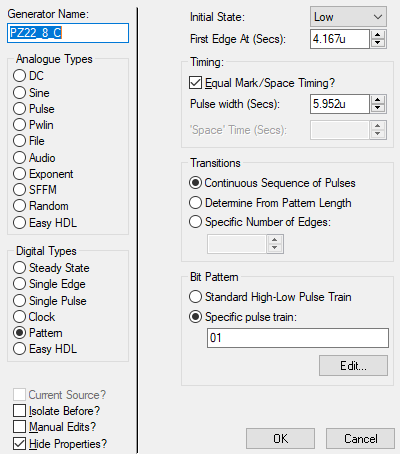
\includegraphics[width=0.45\textwidth]{c}}}
		\hspace{5px}
		\subfloat[Генератор A1]{{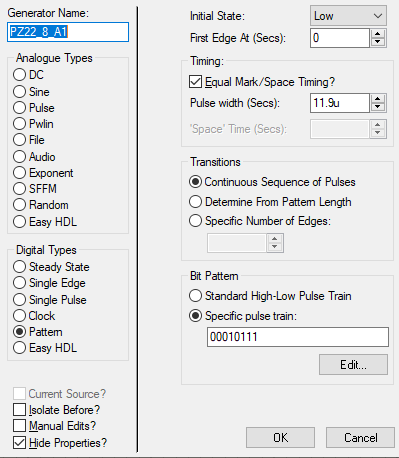
\includegraphics[width=0.45\textwidth]{a1}}}
		
		\subfloat[Генератор A2]{{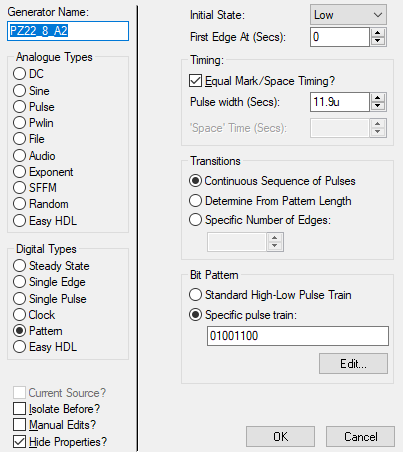
\includegraphics[width=0.45\textwidth]{a2}}}
		\hspace{5px}
		\subfloat[Генератор A3]{{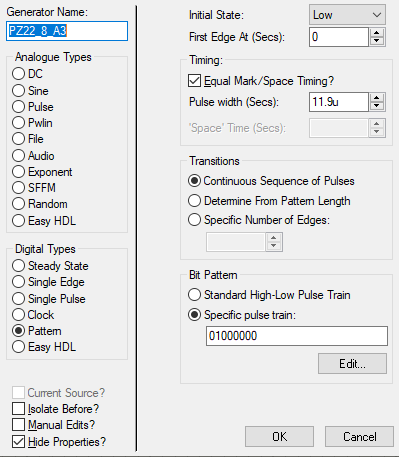
\includegraphics[width=0.45\textwidth]{a3}}}
	\end{figure}

За отриманим графіком виконання схеми паралельного регістра видно, що часові діаграми вхідних та вихідних сигналів відповідають заданому опису функціонування регістра, отже, можна зробити виновок, що моделювання виконано правильно.

	\begin{figure}[H]
		\centering
		\subfloat[Генератор A4]{{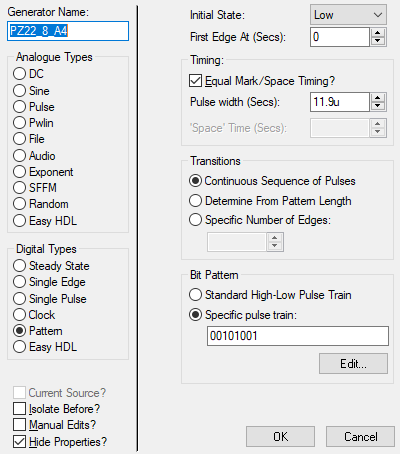
\includegraphics[width=0.45\textwidth]{a4}}}
		\hspace{5px}
		\subfloat[Генератор A5]{{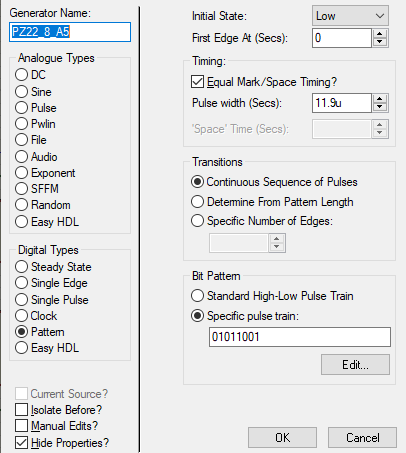
\includegraphics[width=0.45\textwidth]{a5}}}
	\end{figure}

	\section*{5-розрядний регістр зсуву вправо на JK-тригерах}	
	\begin{figure}[H]
		\centering
		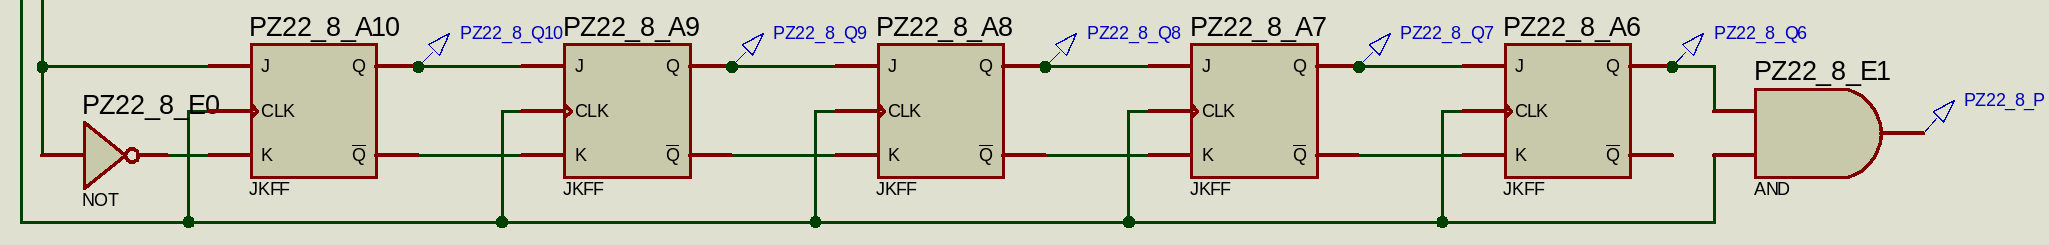
\includegraphics[scale=0.25]{s2}	
		\caption{Схема регістра зсуву}
	\end{figure}
	
	\begin{figure}[H]
		\centering
		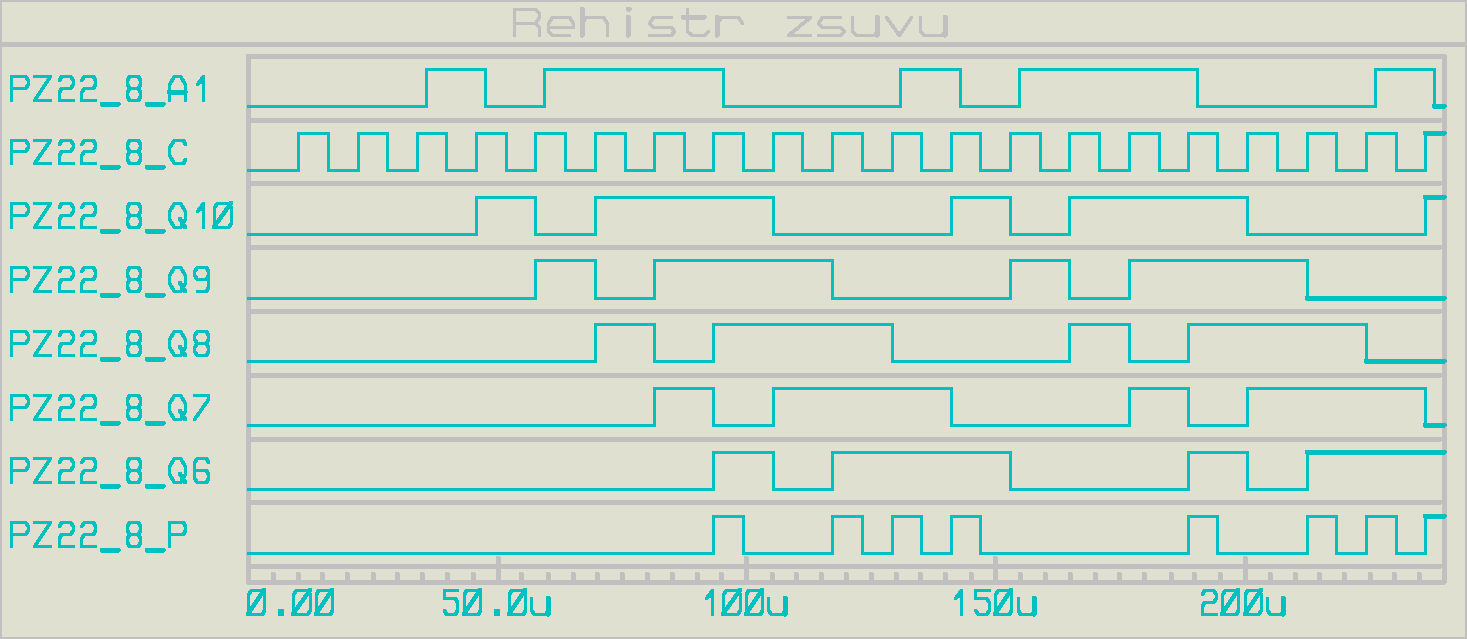
\includegraphics[scale=0.25]{g2}	
		\caption{Графік до схеми регістра зсуву}
	\end{figure}

За отриманим графіком виконання схеми регістра зсуву вправо видно, що часові діаграми вхідних та вихідних сигналів відповідають заданому опису функціонування регістра, отже, можна зробити виновок, що моделювання виконано правильно.

	\begin{figure}[H]
		\centering
		\subfloat[Генератор A1]{{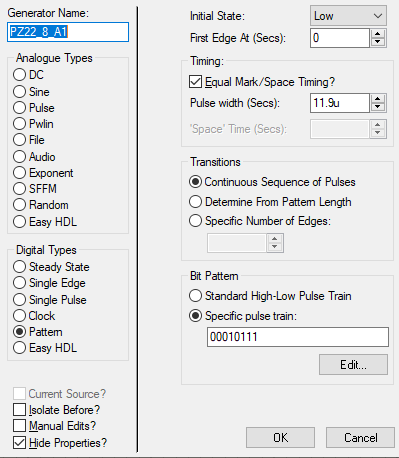
\includegraphics[width=0.45\textwidth]{a1}}}
		\hspace{5px}
		\subfloat[Генератор С]{{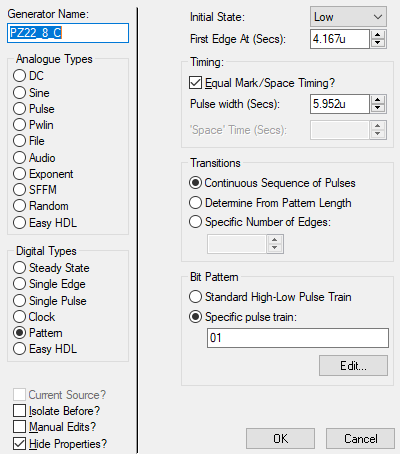
\includegraphics[width=0.45\textwidth]{c}}}
	\end{figure}

	\section*{5-розрядний асинхронний підсумовуючий лічильник на JK-тригерах з прямим динамічним керуванням}	
	\begin{figure}[H]
		\centering
		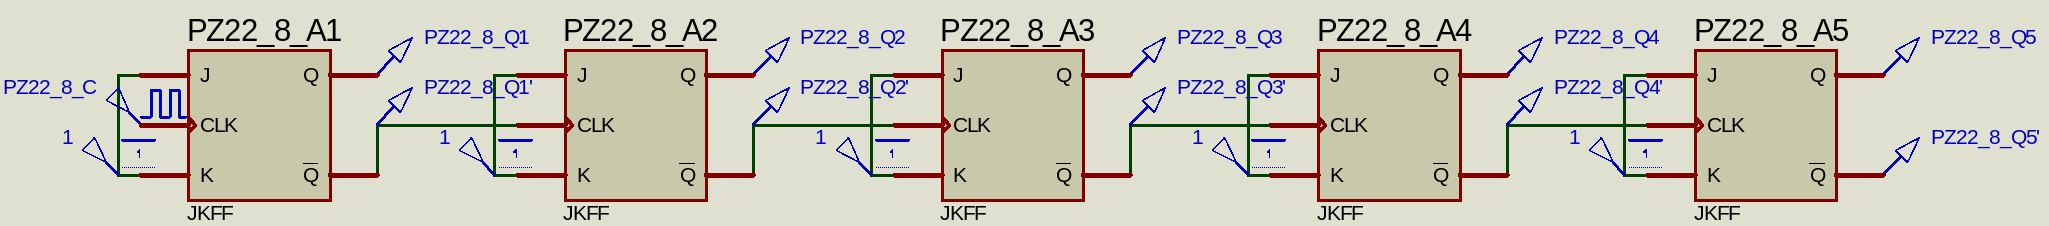
\includegraphics[scale=0.25]{s3}	
		\caption{Схема 5-розрядного асинхронного підсумовуючого лічильника}
	\end{figure}
	
	\begin{figure}[H]
		\centering
		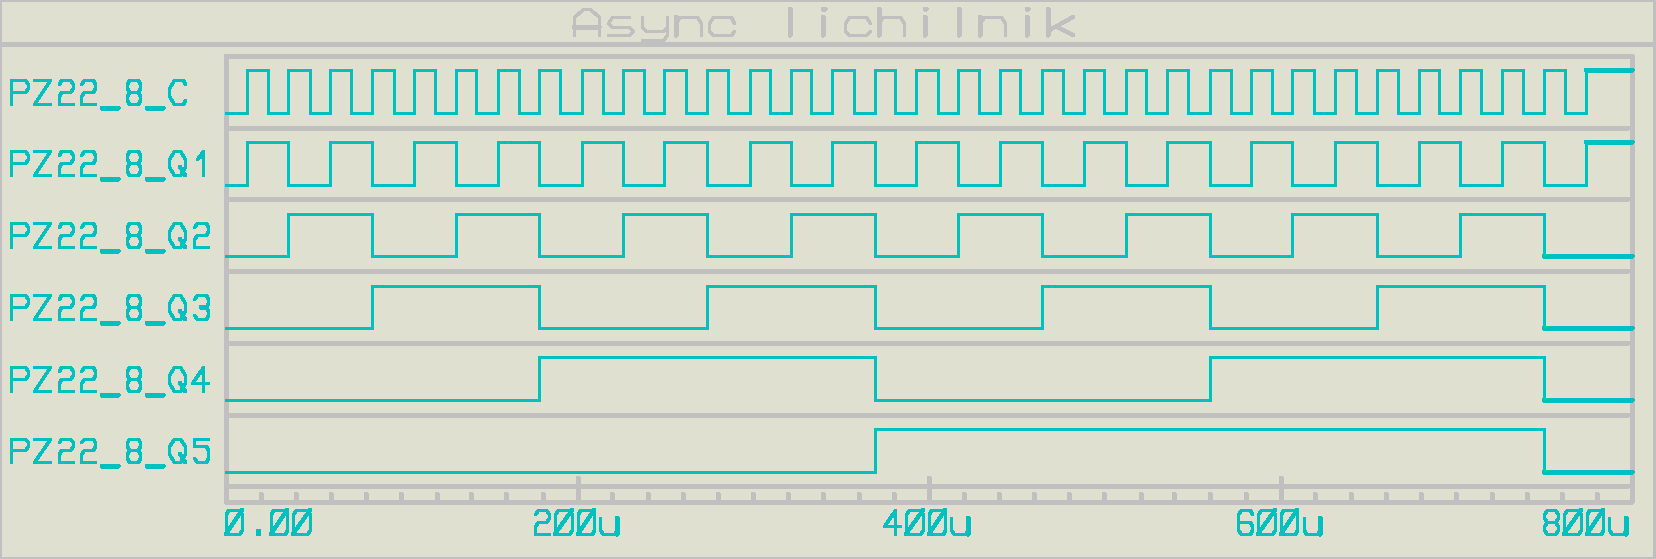
\includegraphics[scale=0.25]{g31}	
		\caption{Графік до схеми 5-розрядного асинхронного підсумовуючого лічильника}
	\end{figure}
	
	\begin{figure}[H]
		\centering
		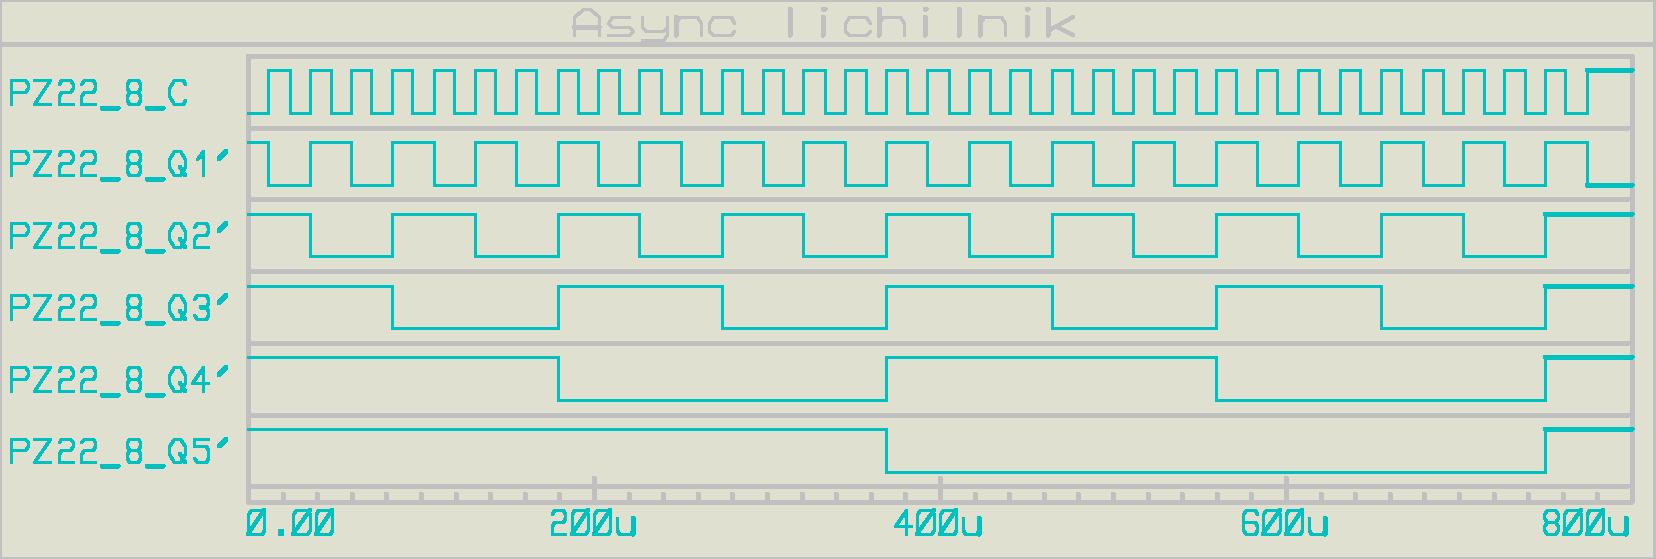
\includegraphics[scale=0.25]{g32}	
		\caption{Графік до схеми 5-розрядного асинхронного підсумовуючого лічильника з оберненим виходом}
	\end{figure}
	
	За отриманим графіком виконання схеми 5-розрядного асинхронного підсумоуючого лічильника  видно, що часові діаграми вхідних та вихідних сигналів відповідають заданому опису функціонування лічильника, отже, можна зробити виновок, що моделювання виконано правильно.
	
	\begin{figure}[H]
		\centering
		\subfloat[Генератор С]{{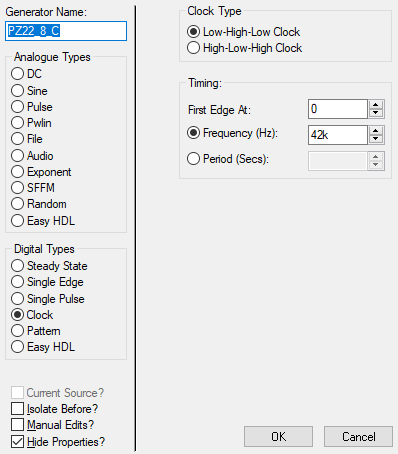
\includegraphics[width=0.45\textwidth]{c2}}}
	\end{figure}

	\section*{5-розрядний асинхронний підсумовуючий лічильник на JK-тригерах з модулем лічби 21}	
	\begin{figure}[H]
		\centering
		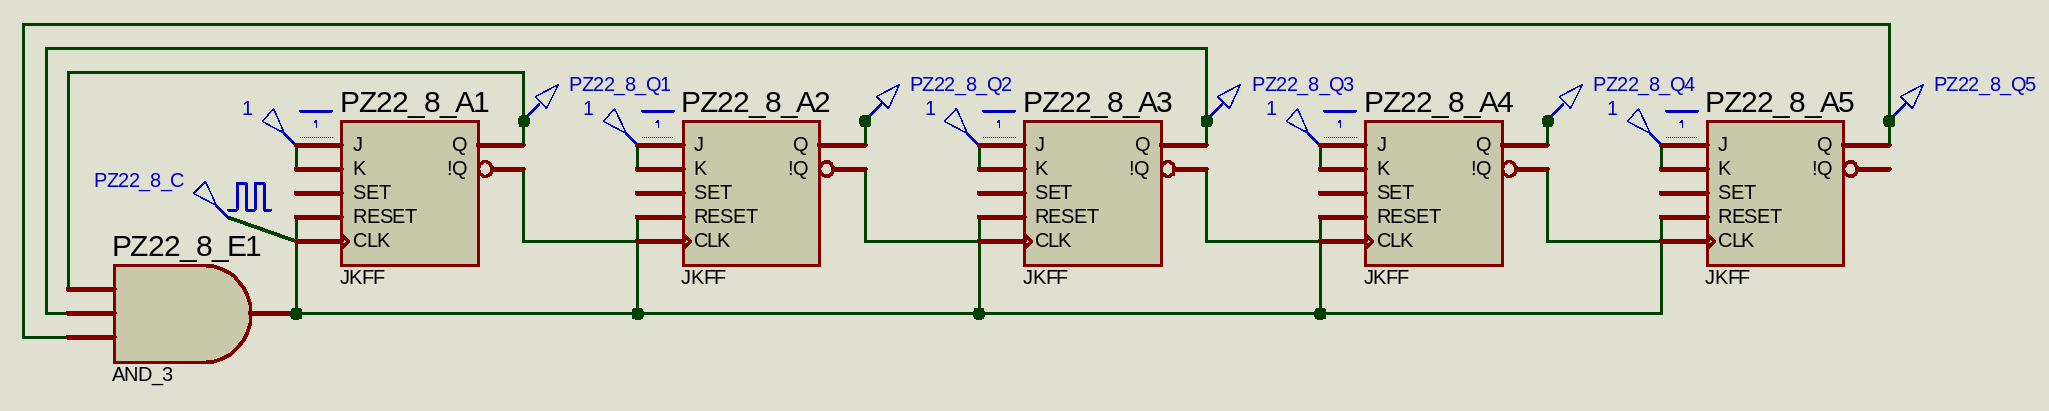
\includegraphics[scale=0.25]{s4}	
		\caption{Схема 5-розрядного асинхронного підсумовуючого лічильника ($M_a=21$)}
	\end{figure}
	
	\begin{figure}[H]
		\centering
		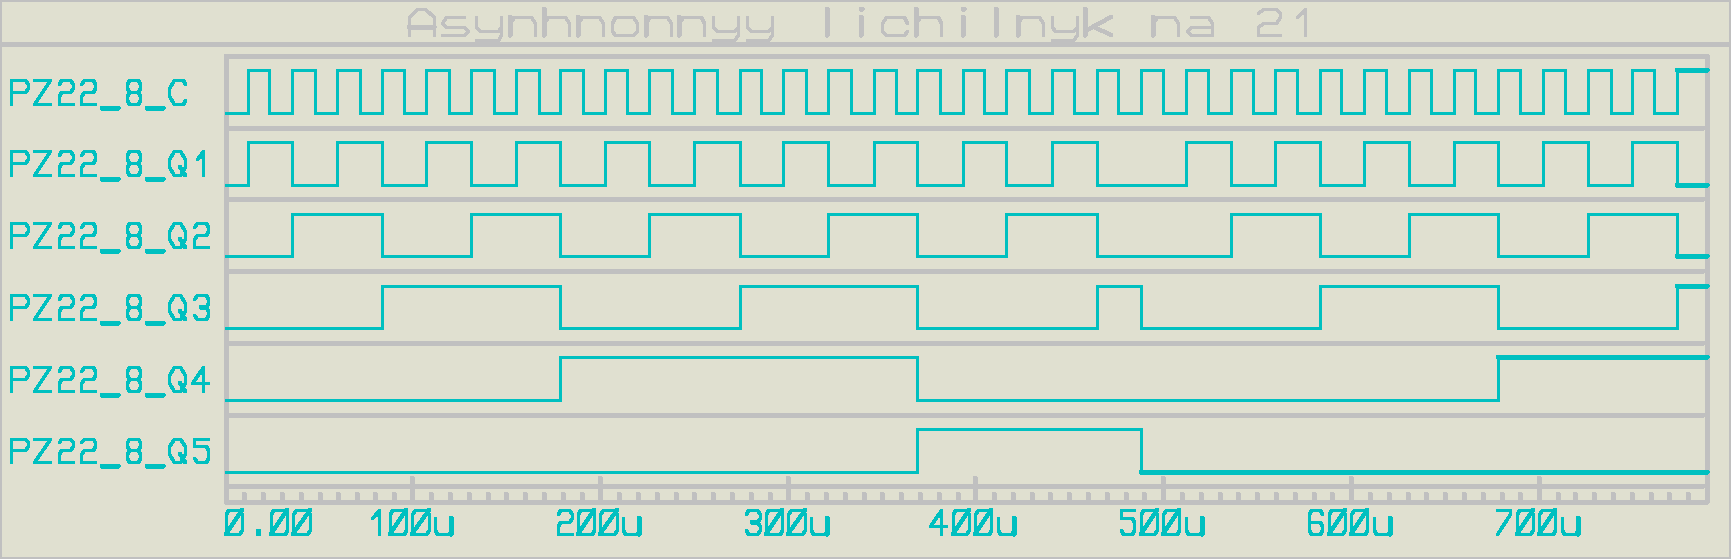
\includegraphics[scale=0.25]{g4}	
		\caption{Графік до схеми 5-розрядного асинхронного підсумовуючого лічильника ($M_a=21$)}
	\end{figure}

За отриманим графіком виконання схеми 5-розрядного асинхронного підсумоуючого лічильника  видно, що часові діаграми вхідних та вихідних сигналів відповідають заданому опису функціонування лічильника, місткість лічби складає 20 (максимальне отримане число), а модуль лічби – 21 (всього різних комбінацій сигналів), отже, можна зробити виновок, що моделювання виконано правильно.
	
	\begin{figure}[H]
		\centering
		\subfloat[Генератор С]{{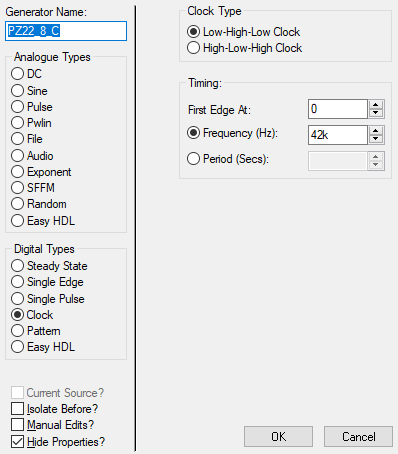
\includegraphics[width=0.45\textwidth]{c2}}}
	\end{figure}
	
	\section*{5-розрядний синхронний підсумовуючий лічильника на JK-тригерах з прямим динамічним керуванням}	
	\begin{figure}[H]
		\centering
		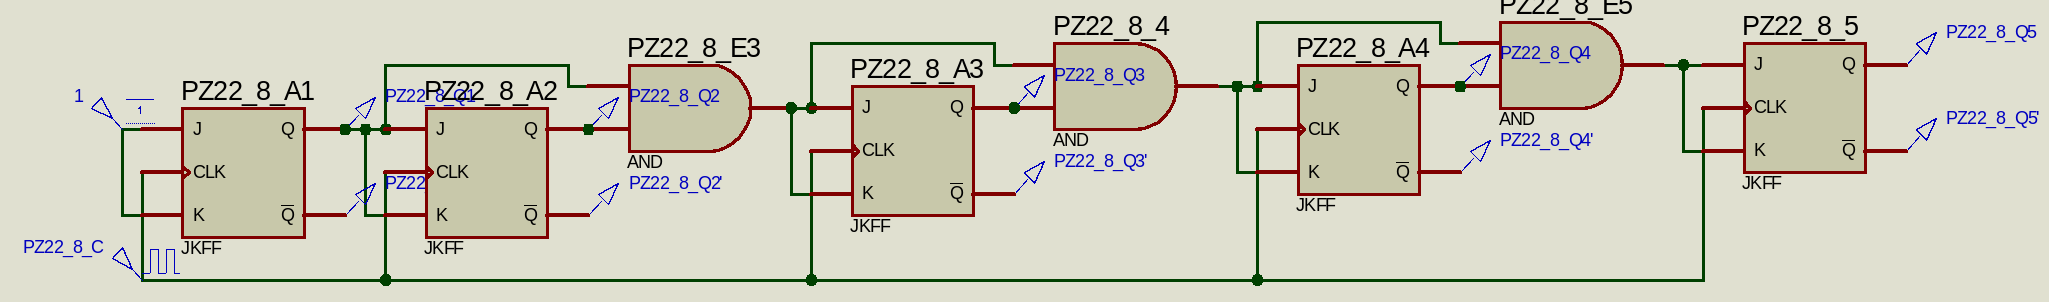
\includegraphics[scale=0.25]{s5}	
		\caption{Схема 5-розрядного синхронного підсумовуючого лічильника}
	\end{figure}
	
	\begin{figure}[H]
		\centering
		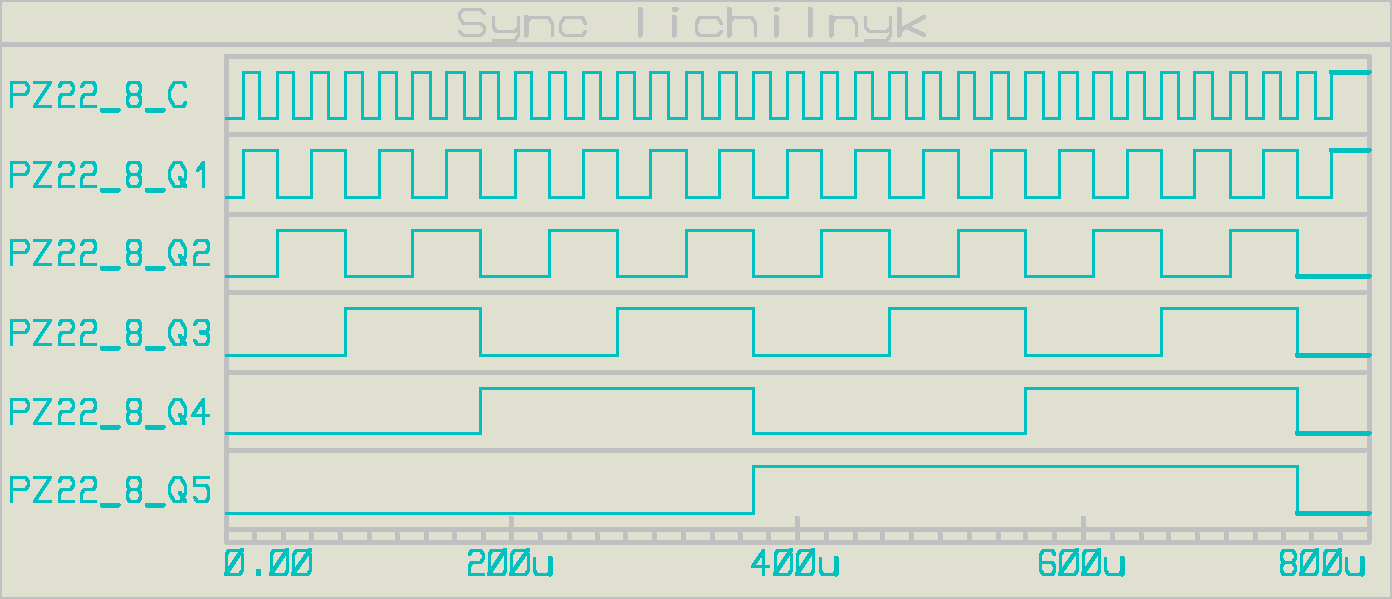
\includegraphics[scale=0.25]{g51}	
		\caption{Графік до схеми 5-розрядного синхронного підсумовуючого лічильника}
	\end{figure}

За отриманим графіком виконання схеми 5-розрядного синхронного підсумоуючого лічильника  видно, що часові діаграми вхідних та вихідних сигналів відповідають заданому опису функціонування лічильника, отже, можна зробити виновок, що моделювання виконано правильно.

	\begin{figure}[H]
		\centering
		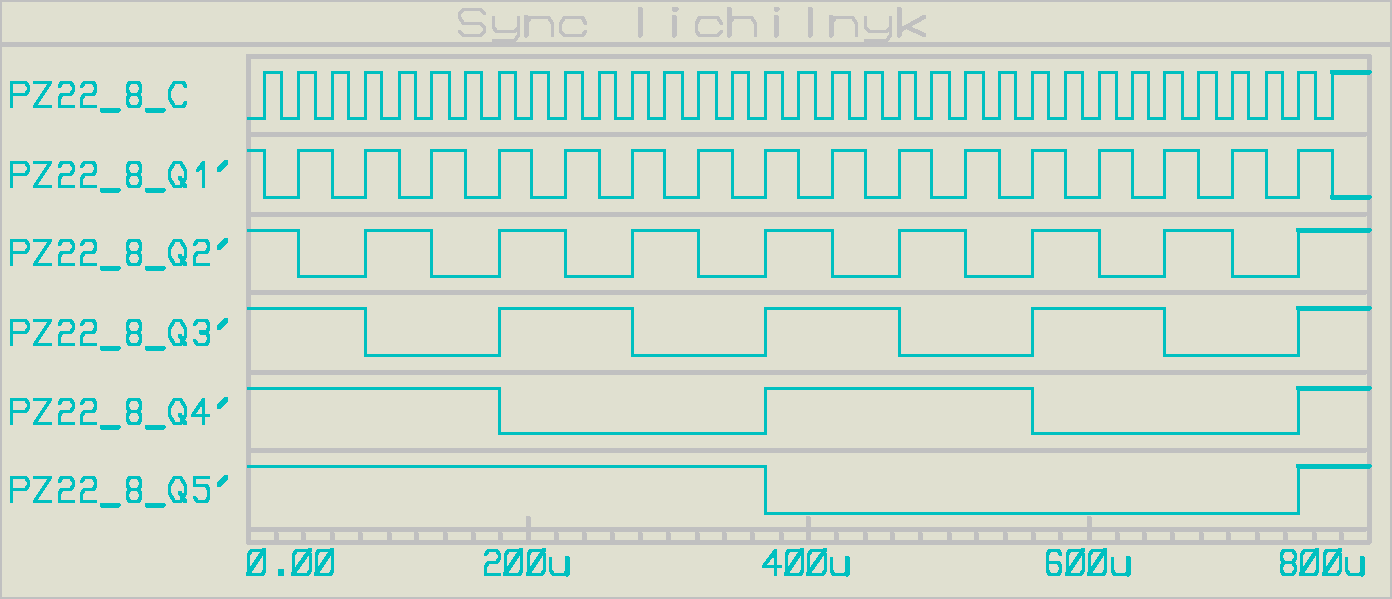
\includegraphics[scale=0.25]{g52}	
		\caption{Графік до схеми 5-розрядного синхронного підсумовуючого лічильника з оберненим виходом}
	\end{figure}
	
	\begin{figure}[H]
		\centering
		\subfloat[Генератор С]{{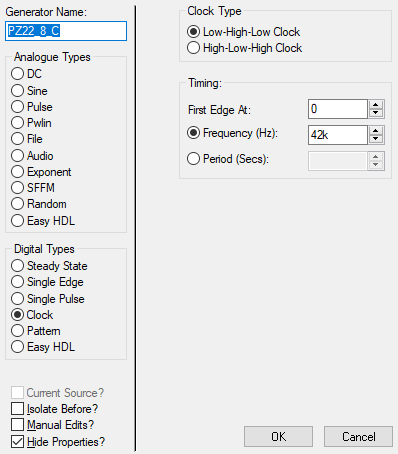
\includegraphics[width=0.45\textwidth]{c2}}}
	\end{figure}

	\section*{5-розрядний синхронний підсумовуючий лічильник на JK-тригерах з модулем лічби 24}	
	\begin{figure}[H]
		\centering
		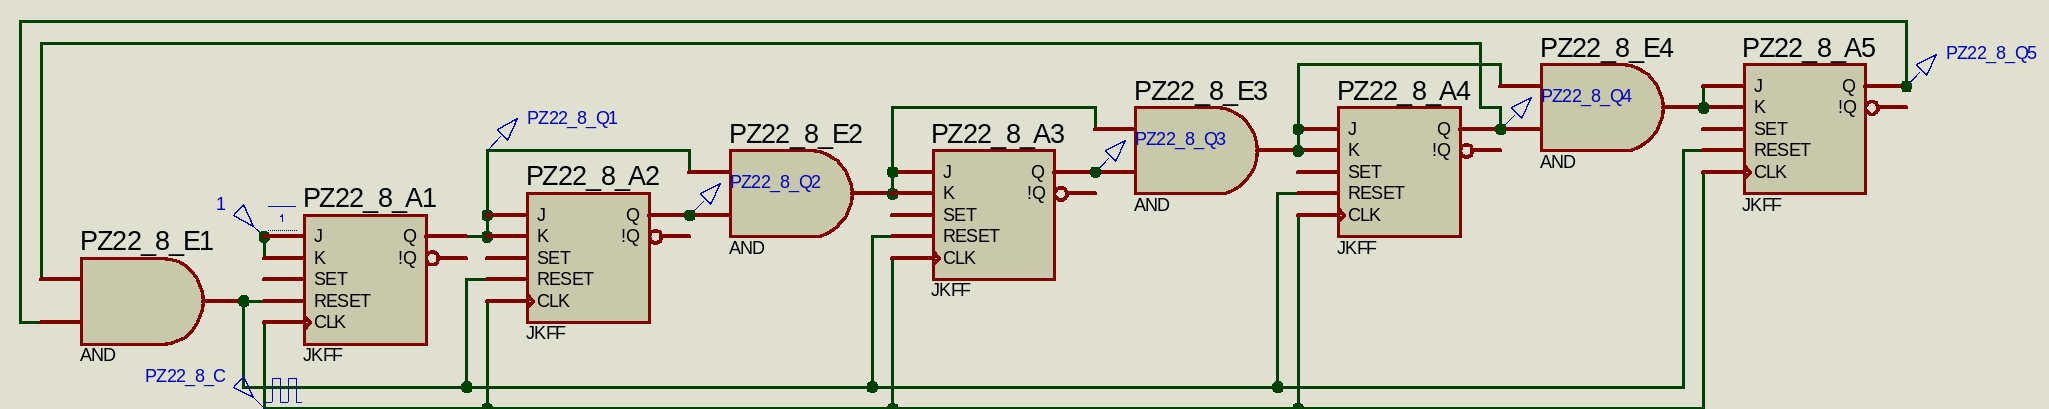
\includegraphics[scale=0.25]{s6}	
		\caption{Схема 5-розрядного синхронного підсумовуючого лічильника ($M_a=24$)}
	\end{figure}
	
	\begin{figure}[H]
		\centering
		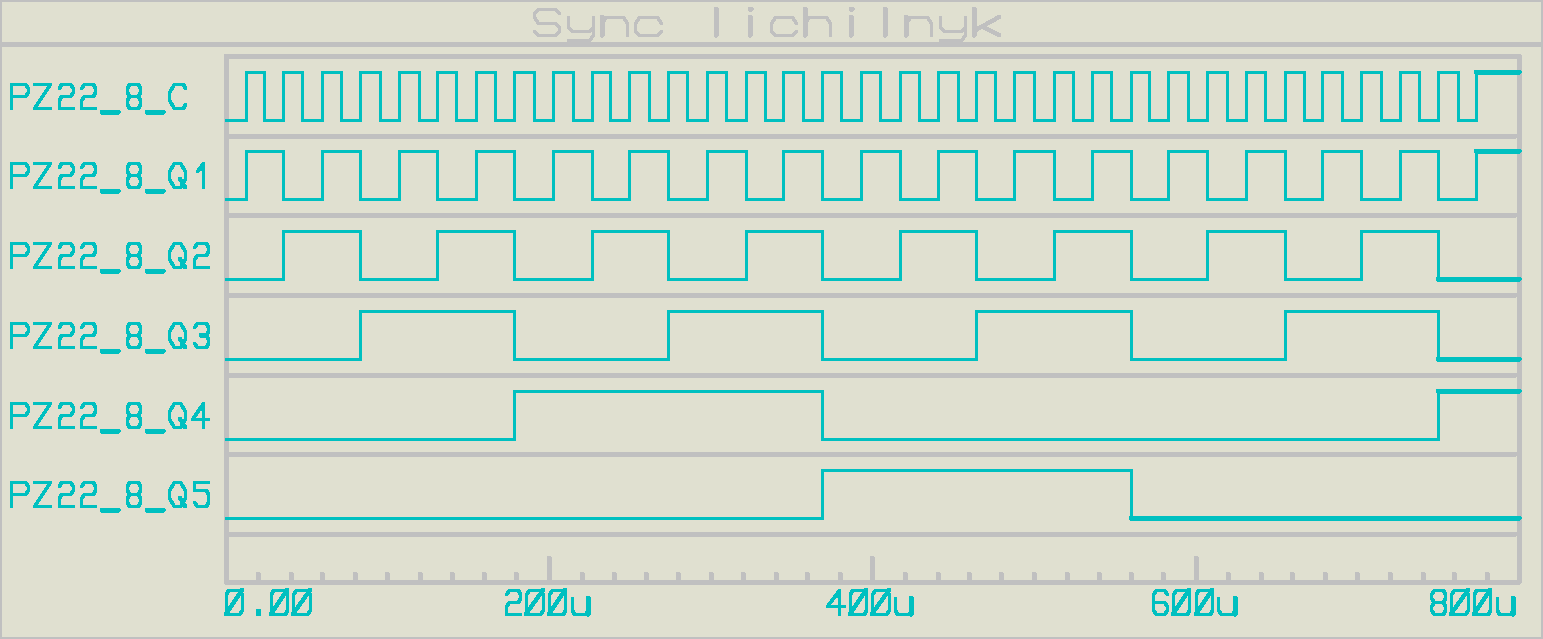
\includegraphics[scale=0.25]{g6}	
		\caption{Графік до схеми 5-розрядного синхронного підсумовуючого лічильника ($M_a=24$)}
	\end{figure}

За отриманим графіком виконання схеми 5-розрядного синхронного підсумоуючого лічильника  видно, що часові діаграми вхідних та вихідних сигналів відповідають заданому опису функціонування лічильника, місткість лічби складає 23 (максимальне отримане число), а модуль лічби – 24 (всього різних комбінацій сигналів)., отже, можна зробити виновок, що моделювання виконано правильно. 
	
	\begin{figure}[H]
		\centering
		\subfloat[Генератор С]{{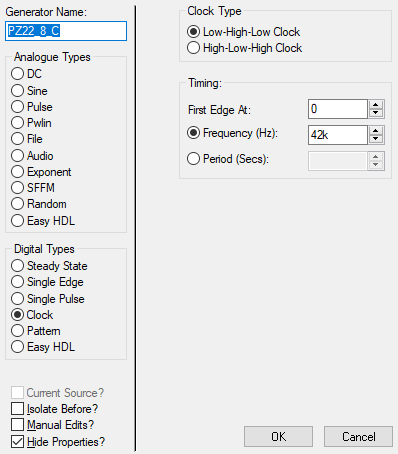
\includegraphics[width=0.45\textwidth]{c2}}}
	\end{figure}

	\section*{Висновки}
	Під час виконання лабораторної роботи я поглибив знання про будову та функціонування основних типів регістрів та лічильників; синтезував їх схеми та виконав моделювання в системі програм Proteus; дослідив на основі отриманих часових діаграм їх роботу. 
	
	Дослідив роботу синтезованих схем в системі програм Proteus. Змоделював графіки цих схем за заданим варіантом.
	    
\end{normalsize}
\end{document}
